\documentclass[../main.tex]{subfiles}

\begin{document}

\chapter{Avaliação}\label{cap:avaliacao}

Com o objetivo de avaliar a abordagem BumbAR, foi desenvolvido um estudo empírico qualitativo no qual os participantes desenvolveram uma apresentação multimídia utilizando a ferramenta. A seguir, eles são convidados a preencher um questionário com suas percepções sobre a ferramenta de autoria. O principal objetivo desse estudo é analisar a atitude dos usuários em relação à criação de apresentações multimídia utilizando a ferramenta desenvolvida e, de maneira mais geral, uma interface baseada em realidade aumentada para a criação de tais apresentações.

No restante deste capítulo, são detalhadas a metodologia utilizada (Seção \ref{sec:metodologia}), o perfil dos participantes (Seção \ref{sec:participantes}), e os resultados da avaliação (Seção \ref{sec:resultados}).

\section{Metodologia de Avaliação}
\label{sec:metodologia}

O estudo empírico desenvolvido para avaliar a ferramenta BumbAR constituiu-se de cinco fases distintas. Tais fases são mostradas na Figura~\ref{fig:metodologia_exp} e são detalhadas a seguir.

\begin{figure}[!h]
\centering
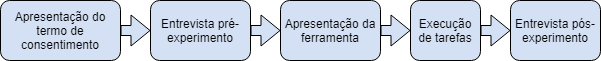
\includegraphics[width=0.9\linewidth]{IMG/metodologia_experimento.png}
\caption{Fases metodológicas do estudo.}
\fonte{Elaborada pelo autor.}
\label{fig:metodologia_exp}
\end{figure}


\begin{itemize}
    \item \textbf{Apresentação do termo de consentimento:} O termo de consentimento é apresen-tado, enfatizando verbalmente os objetivos desta pesquisa. O participante é convidado a consentir ou não em participar desta pesquisa, assinando o termo de consentimento em caso positivo.
    \item \textbf{Entrevista pré-experimento:} O objetivo dessa fase é elaborar o perfil do participan-te, especialmente sobre seu conhecimento em relação à realidade aumentada e apresentações multimídia.
    \item \textbf{Apresentação da ferramenta:} O objetivo dessa fase é apresentar os conceitos essenciais da ferramenta BumbAR, e como compor apresentações multimídia com ela.
    \item \textbf{Execução de tarefas:} O participante é convidado a ler o cenário. Após isso, a apresentação multimídia é tocada, enfatizando o comportamento esperado desta. Finalmente, o participante é convidado a compor, utilizando a ferramenta BumbAR, uma apresentação multimídia igual à que lhe foi apresentada.
    \item \textbf{Entrevista pós-experimento:} O objetivo desta fase é colher as percepções dos participantes em relação às tarefas executadas, e as facilidades e dificuldades encontradas ao usar a ferramenta BumbAR.
\end{itemize}

As tarefas da fase de \emph{execução de tarefas} objetivaram a composição de uma apresentação multimídia composta por quatro vídeos. A Figura \ref{fig:expected_presentation} mostra o comportamento esperado da apresentação a ser desenvolvida pelos participantes.

\begin{figure}[!h]
\centering
  \begin{subfigure}[t]{0.31\linewidth}
    
\includegraphics[width=0.98\linewidth]{IMG/Avaliacao/exp1.png}
    \caption{Apresentando o vídeo 1 assim que a apresentação inicia.}
  \end{subfigure}\hspace{0.02\linewidth}
  \begin{subfigure}[t]{0.31\linewidth}
    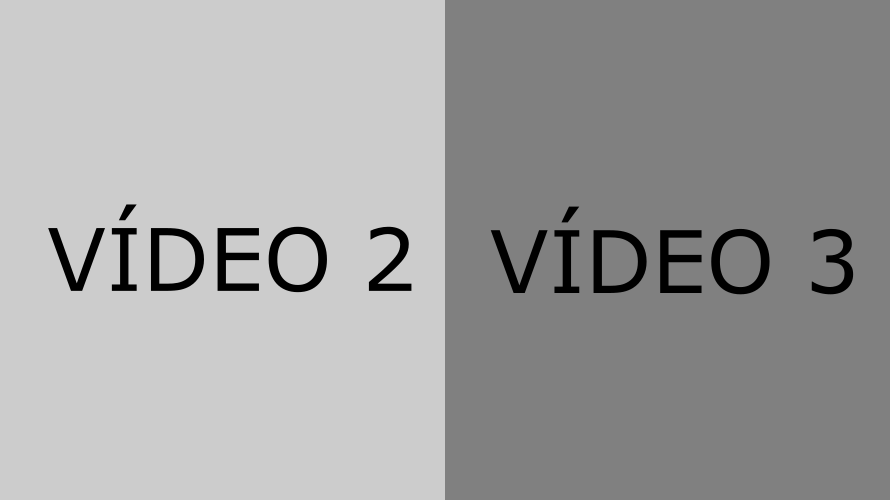
\includegraphics[width=0.98\linewidth]{IMG/Avaliacao/exp2.png}
    \caption{Apresentando os vídeos 2 e 3 simultaneamente.}
  \end{subfigure}\hspace{0.02\linewidth}
  \begin{subfigure}[t]{0.31\linewidth}
    
\includegraphics[width=0.98\linewidth]{IMG/Avaliacao/exp3.png}
    \caption{Apresentando o vídeo 4 depois de os vídeos 2 e 3 acabarem.}
  \end{subfigure}
\caption{Apresentação resultante esperada do experimento.}
\fonte{Elaborada pelo autor.}
\label{fig:expected_presentation}
\end{figure}

Os passos necessários parara compor essa apresentação foram divididos em quatro tarefas. Tais tarefas foram mostradas em um monitor para que os participantes as pudessem seguir, e são as seguintes:

\begin{itemize}
    \item \textbf{Tarefa 1:} Configure quatro vídeos em volume máximo possuindo as seguintes configurações:
    \begin{itemize}
        \item vídeo~1: possui a URL \emph{video1.mp4} e ocupa a tela inteira;
        \item vídeo~2: possui a URL \emph{video2.mp4} e ocupa a metade esquerda da tela;
        \item vídeo~3: possui a URL \emph{video3.mp4} e ocupa a metade direita da tela;
        \item vídeo~4: possui a URL \emph{video4.mp4} e ocupa a tela inteira;
    \end{itemize}
    \item \textbf{Tarefa 2:} Faça uma apresentação multimídia que toque o vídeo~1;
    \item \textbf{Tarefa 3:} Estenda a apresentação multimídia desenvolvida na tarefa 2 para fazer o seguinte: quando o vídeo~1 terminar, toque dois outros vídeos, vídeo~2 e vídeo~3, ao mesmo tempo;
    \item \textbf{Tarefa 4:} Estenda a apresentação multimídia desenvolvida na tarefa 3 para fazer o seguinte: quando o vídeo~2 terminar, pare o vídeo 3 e toque o vídeo~4;
\end{itemize}

Para desenvolver a apresentação, os participantes utilizaram uma instalação de realidade aumentada composta por um notebook, com a ferramenta BumbAR, uma webcam, e os marcadores de realidade aumentada utilizados pela ferramenta. Os marcadores foram restritos ao marcador \emph{inicial}, marcadores de \emph{condição}, marcadores de \emph{ação} e quatro marcadores de \emph{mídia}.

Para fase de entrevista pós-experimento, foi desenvolvido um questionário baseado no modelo de aceitação de tecnologias, do inglês \emph{Technology Acceptance Model}(TAM)~\cite{davis1985technology,
davis1989user, venkatesh2000theoretical, davis_perceived_1989}, que é amplamente utilizado para avaliar a aceitação de novas tecnologias~\cite{wojciechowski2013evaluation, alraimi2015understanding,
pavlou2003consumer}. O modelo TAM propõe sentenças baseadas em dois conteitos: utilidade percebida, do inglês \emph{perceived usefulness}(PU), e facilidade de uso percebida, do inglês \emph{perceived ease-of-use}(PEOU). \citeonline{davis1989user} definem PU como o nível em que uma pessoa percebe que o uso de um sistema melhoraria sua performance em fazer seu trabalho, e PEOU como o nível em que uma pessoa acredita que o uso de um sistema seria livre de esforço.

A Tabela~\ref{tab:tam_sentencas} mostra o questionário desenvolvido para a avaliação qualitativa do experimento, instanciado a partir do TAM para o presente contexto. Tal questionário é composto de sete sentenças do tipo PU, sete do tipo PEOU e duas questões livres para os participantes darem opiniões sobre a ferramenta. Cada sentença possui opções baseadas em uma escala Likert de sete pontos~\cite{vagias2006likert} com as seguintes opções: 1 - discordo totalmente; 2 - discordo; 3 - discordo um pouco; 4 - nem discordo nem concordo; 5 - concordo um pouco; 6 - concordo; 7 - concordo totalmente.

\begin{table*}[htpb]
\caption{Questionário baseado no modelo TAM usado na avaliação da proposta.}
\label{tab:tam_sentencas}
\begin{tabularx}{.95\linewidth}{m{1.3cm} X}
\toprule
 & \textbf{\centering Sentenças do Questionário}
\\\otoprule
PU1 & Em geral, os conceitos apresentados (objetos de mídia, elos, condições, e ações) são úteis para criar apresentações multimídia.
\\\midrule
PU2 & Em geral, o desenvolvimento de apresentações multimídia usando realidade aumentada é útil.
\\\midrule
PU3 & Em geral, o processo de desenvolvimento de apresentações multimídia usando Realidade Aumentada com os marcadores escolhidos é útil.
\\\midrule
PU4 & Eu considero que a ferramenta é mais simples de usar em relação a outras que conheço.
\\\midrule
PU5 & Eu acredito que a ferramenta torna o desenvolvimento de apresentações multimídia rápido.
\\\midrule
PU6 & Eu acredito que a ferramenta é útil.
\\\midrule
PU7 & Em geral, eu acredito que a ferramenta é vantajosa.
\\\midrule
PEOU1 & Em geral, o processo de autoria com realidade aumentada é simples e compreensível.
\\\midrule
PEOU2 & Em geral, o processo de autoria com realidade aumentada com os marcadores escolhidos é simples e compreensível
\\\midrule
PEOU3 & Em geral, o modelo adotado para o sincronismo de objetos de mídia (elos, condições, ações) é simples e compreensível.
\\\midrule
PEOU4 & Aprender a usar a ferramenta foi fácil para mim.
\\\midrule
PEOU5 & Na minha opinião, a ferramenta é fácil de usar.
\\\midrule
PEOU6 & Na minha opinião, a ferramenta deixa o desenvolvimento de apresentações multimídia fácil.
\\\midrule
PEOU7 & Eu acredito que eu poderia me tornar habilidoso no desenvolvimento de apresentações multimídia com a ferramenta.
\\\midrule
Livre1 & Cite pontos positivos da ferramenta, se existirem.
\\\midrule
Livre2 & Cite pontos negativos da ferramenta, se existirem.
\\\bottomrule
\end{tabularx}
\end{table*}

\section{Participantes}
\label{sec:participantes}

O experimento envolveu estudantes universitários dos cursos de Ciência da Computa-ção e Design da Universidade Federal do Maranhão. Esse grupo foi escolhido porque o desenvolvimento de aplicações multimídia é frequentemente presente no currículo desses profissionais. Um total de 15 estudantes com idades variando de 20 a 27 anos participaram do experimento de avaliação.

O grau de conhecimento dos participantes tanto no desenvolvimento de apresentações multimídia quanto em realidade aumentada foi levado em consideração. Tal grau de conhecimento foi medido em uma escala Likert de sete pontos variando de 1~(Nenhum) a 7~(Especialista).

A Tabela \ref{tab:expParticipantes} mostra a quantidade de participantes que escolheram cada uma das opções.

\begin{table}[ht!]
\caption{Grau de conhecimento dos participantes do experimento.}
\label{tab:expParticipantes}

\begin{tabular}{@{}ccc@{}}
\toprule
\textbf{Grau de Conhecimento} & \textbf{Apresentações Multimídia} & \textbf{Realidade Aumentada} \\ \midrule
Nenhum                        & 3                                 & 0                            \\
Muito Pouco                   & 3                                 & 0                            \\
Pouco                         & 2                                 & 2                            \\
Mediano                       & 5                                 & 10                           \\
Alto                          & 2                                 & 3                            \\
Muito Alto                    & 0                                 & 0                            \\
Especialista                  & 0                                 & 0                            \\ \bottomrule
\end{tabular}
\end{table}

\section{Resultados}
\label{sec:resultados}

Não houveram problemas técnicos durante a condução do experimento, de modo que os participantes puderam focar nos méritos deste. Todos os participantes completaram as tarefas propostas e, consequentemente, desenvolveram a apresentação multimídia solicitada. O tempo médio de desenvolvimento foi de 13 minutos e 49 segundos, com um desvio padrão de 3 minutos e 17 segundos.

Para calcular a consistência interna dos dados colhidos, foi calculado o coeficiente alfa de Cronbach dos dois grupos de sentenças, PU e PEOU. Tal coeficiente é calculado de acordo com a fórmula:

\[\alpha = \frac{k}{k-1}\Bigg(1 - \frac{\sum_{i = 1}^{k}S_i^2}{S_{soma}^2}\Bigg)\]

Onde \(k\) é o número de itens do questionário, \(S_i^2\) é a variância para o i-ésimo item \((i=1,...k)\), \(S_{soma}^2\) é a variância das somas das respostas de cada participante.

O coeficiente das sentenças PU encontrado foi de 0,7637, enquanto que para as sentenças PEOU foi de 0,8433. Um coeficiente alfa de Cronbach maior que 0,7 geralmente indica que a confiabilidade das sentenças está em um nível satisfatório. 

A Figura \ref{fig:resultados} mostra as respostas para cada sentença em valores absolutos e em percentual. Todas as sentenças obtiveram a maioria de suas respostas positivas. A sentença PU6, que diz "eu acredito que a ferramenta é útil", e PEOU5, que diz "na minha opinião, a ferramenta é fácil de usar", obtiveram um nível significante de concordâncias, com respostas 5~(concordo um pouco) ou superior. Esses resultados revelam que, na opinião dos participantes, a ferramenta que utiliza o processo proposto é útil e fácil de usar.

\begin{figure*}[ht!]
\centering
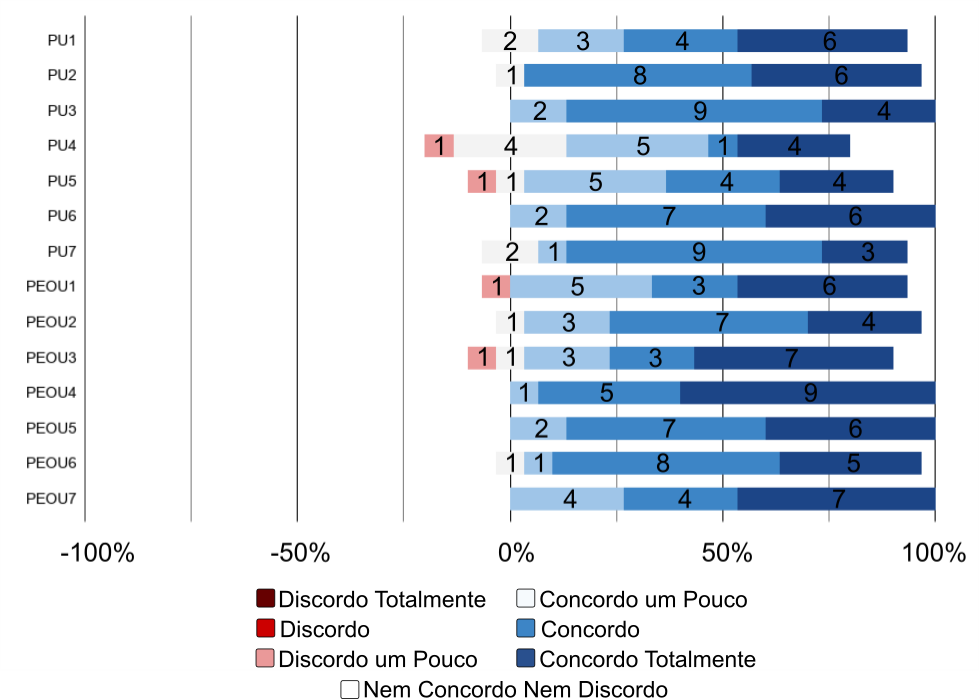
\includegraphics[width=0.8\textwidth]{IMG/Avaliacao/resultados_bumbar.png}
\caption{Respostas dos participantes sobre a ferramenta BumbAR}
\fonte{Elaborada pelo autor.}
\label{fig:resultados}
\end{figure*}

Como mencionado anteriormente, também foram considerados comentários dos participantes sobre pontos positivos e negativos da ferramenta. De fato, os comentários dos participantes se mostraram relevantes, e seriam perdidos em um experimento puramente quantitativo. Do lado positivo, a maioria dos participantes mencionou a intuitividade da ferramenta BumbAR e que ela torna o processo de autoria agradável. Do lado negativo, a maioria dos participantes enfatizou a necessidade de mostrar o histórico de elos criados, o que motivou a criação do \emph{marcador de visão estrutural} e do \emph{marcador de elos}, descritos na Seção \ref{subsec:criacao_elos}.

Um dos participantes do experimento comentou que a ferramenta BumbAR "é mais rápida e menos complicada que outros métodos". De acordo com resultados colhidos, a maioria dos participantes concorda com essa afirmação: $86,67\%$ dos participantes acredita que a ferramenta torna o desenvolvimento de apresentações mais rápido, enquanto $66,67\%$ consideram ela mais conveniente quando comparada com ferramentas tradicionais.

\end{document}